\documentclass[11pt,a4paper,roman]{scrartcl}
\usepackage{parskip}
\usepackage[english]{babel}
\usepackage{url}
\usepackage[utf8x]{inputenc}
\usepackage{amsmath}
\usepackage{amssymb}
\usepackage{graphicx}
\usepackage[export]{adjustbox}
\usepackage{listings}
\usepackage{float}
\usepackage{hyperref}
\usepackage[document]{ragged2e}
\usepackage{bm}
\usepackage[section]{placeins}
\title{Computer exercise 6}
\date{}
\author{Carl Ridnert, 940325-0112, ridnert@kth.se \\
Yue Jiao, 911024-7799, yj@kth.se}

\begin{document}

\maketitle
\begin{figure}[h]
\centering
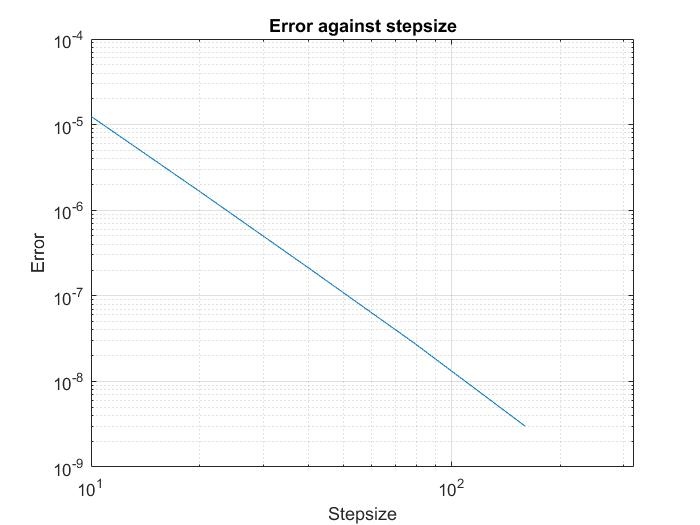
\includegraphics[width=0.45\textwidth,center]{1}
\end{figure}


\newpage

\section*{Problem 1}
\subsection*{Analysis}
In this problem the hyperbolic PDE problem is treated numerically. The PDE is the following: 
\begin{equation}
\frac{\partial u}{\partial t} + a\frac{\partial u}{\partial x} = 0
\end{equation}
with IC $u(x,0)=0, 0<x\leq 2$ and the following boundary condition:
\begin{equation}
u(0,t) = \begin{cases}
1, \quad & n\frac{T}{2} < t \leq (n+1)\frac{T}{2},  \\
-1, \quad & (n+1)\frac{T}{2} < t \leq (n+2)\frac{T}{2}, \\
\end{cases} \quad n = 0,2,4,\dots
\end{equation}

The space is discretized into $N$ equidistant subintervals and define grid points $x_i = ih_x$ where $h_x = 2/N$ and the Courant number $\sigma$ to be used later is defined as $\sigma = ah_t/h_x$. 

\subsection*{Solving with upwind method}
With the upwind method the PDE is discretized into the following form:
\begin{equation}
u_{i,k+1} = (1-\sigma) u_{i,k} + \sigma u_{i-1,k}
\end{equation}
This method is stable when $0<\sigma \leq 1$ and thus it performs well when $\sigma = 1$. 

\subsection*{Solving with Lax-Friedrich method}
With the upwind method the PDE is discretized into the following form:
\begin{equation}
\begin{aligned}
u_{i,k+1} & = \frac{u_{i-1,k}+u_{i+1,k}}{2}- \frac{\sigma}{2}(u_{i+1,k}-u_{i-1,k}) \\
u_{N, k+1} & = 2u_{N-1, k+1} - u_{N-2, k+1}
\end{aligned}
\end{equation}
According to the theory, the method is stable when $-1\leq \sigma \leq 1$.

\subsection*{Solving with Lax-Wendroff method}
With the upwind method the PDE is discretized into the following form:
\begin{equation}
\begin{aligned}
u_{i,k+1} & = u_{i,k}-\frac{\sigma}{2}(u_{i+1,k}-u_{i-1,k})+\frac{\sigma^2}{2}(u_{i+1,k}-2u_{i,k}+u_{i-1,k}) \\
u_{N, k+1} & = 2u_{N-1, k+1} - u_{N-2, k+1}
\end{aligned}
\end{equation}
According to the theory, the method is stable when $-1\leq \sigma \leq 1$.
\newpage
The PDE was solved in Matlab using each of the three methods described above for sigma taking the values $\sigma\in\{0.8,1,1.1\}$ and the resulting plots of the solution is shown below.


\begin{figure}[!h]
\centering
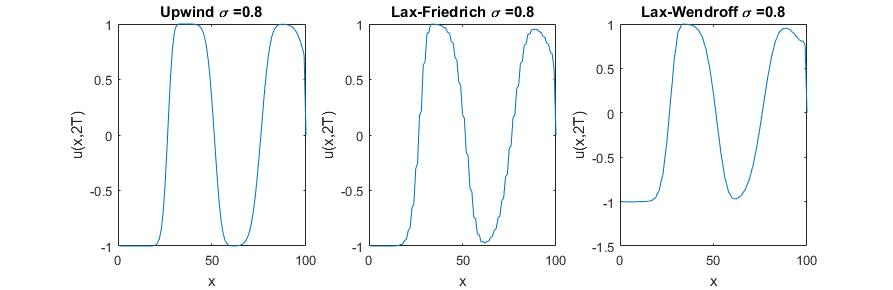
\includegraphics[width=1.2\textwidth,center]{Subplot1}
\caption{Plots of solutions using different methods when $\sigma=0.8$}
\end{figure}

\begin{figure}[!h]
\centering
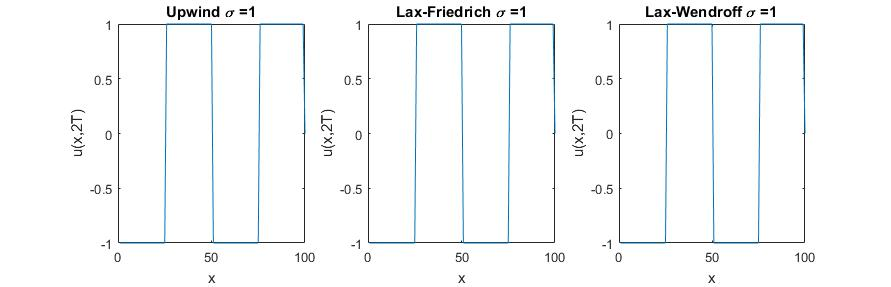
\includegraphics[width=1.2\textwidth,center]{Subplot2}
\caption{Plots of solutions using different methods when $\sigma=1$}
\end{figure}

\begin{figure}[!h]
\centering
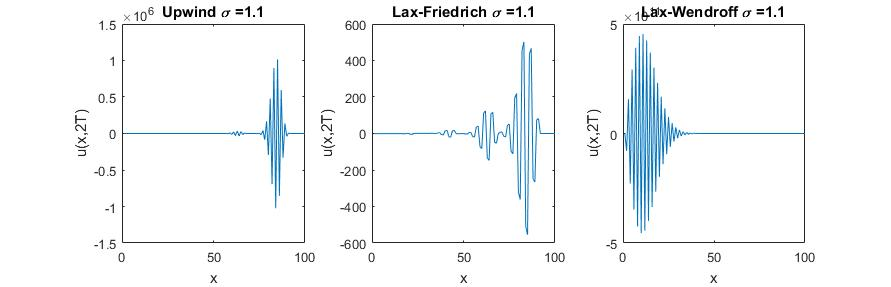
\includegraphics[width=1.2\textwidth,center]{Subplot3}
\caption{Plots of solutions using different methods when $\sigma=1.1$}
\end{figure}
\FloatBarrier
Notice that the solutions become unstable when $\sigma$ is larger than one. For $\sigma=1$ the function in the boundary condition is preserved and propagated along the time axis. This is in agreement with the theory presented above. Lax-Friedrich method introduces some non-smoothness which is not present when using upwind method. Finally we note that Lax-Wendroff seems to give spurious oscillations, this is a consequence of using a second order discretization in time but not in x. 

\section*{Problem 2}
\subsection*{Analysis}
In this problem the following PDE is solved:
\begin{equation}
\frac{\partial T}{\partial t} + \nu\frac{\partial T}{\partial x}+a(T-T_{cool}) = 0, \quad 0<x<L, \quad t>0
\end{equation}
with the IC: 
\begin{equation}
T(x,0)=T_{cool}
\end{equation}
and the BC:
\begin{equation}
T(0,t) = 
\begin{cases}
T_{cool} + (T_{hot}-T_{cool})sin(\pi t) \quad & 0\leq t \leq 0.5 \\
T_{hot}	\quad & 0.5 \leq t \leq 4 \\
T_{hot} + T_{cool} sin(\pi(t-4)) \quad & t>4\\
\end{cases}
\end{equation}
Here we have the parameters $L=3$, $a=0.1$, $\nu=1$, $T_{cool}=5$ and $T_{hot} = 100$.

\subsection*{Solving with upwind method}
To let the upwind method perform in the best way, we want to choose $h_x$ and $h_t$ so that $\sigma = \nu h_t/h_x=1$. We choose to divide the region into 30 equidistant subintervals so $h_x=L/30=0.1$ and then $h_t = \sigma h_x /\nu =0.1$

Then the PDE can be discretized into the following form: 
\begin{equation}
\frac{T_{i,k+1}-T_{i,k}}{h_t}+\nu\frac{T_{i+1,k}-T_{i-1,k}}{2h_x} + a(T_{i,k}-T_{cool}) = 0
\end{equation}
With $i$ indexes the discretization of $x$-axis and $k$ indexes the discretization to the time-axis. This formula can be rewritten as the following: 
\begin{equation}
T_{i,k+1} = (1-ah_t)T_{i,k}-\frac{1}{2}(T_{i+1,k}-T_{i-1,k})+ah_tT_{cool}
\end{equation}
The IC shall become: 
\begin{equation}
T_{i,1} = T_{cool} 
\end{equation}

This was solved in Matlab and the results is presented below.

\begin{figure}[!h]
\centering
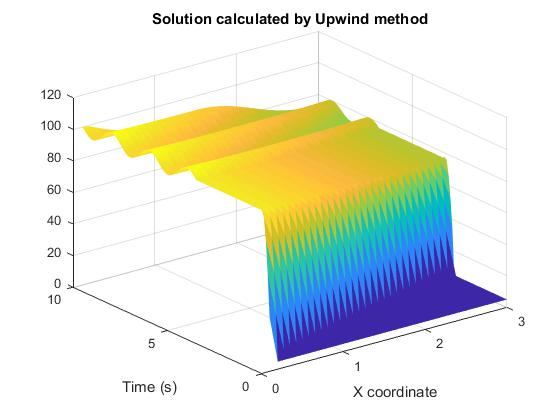
\includegraphics[width=\textwidth,center]{surf1}
\caption{Plots of solution using the Upwind method}
\end{figure}

\newpage
\subsection*{Solving with The Lax–Wendroff Method}
The Lax-Wendroff method is based on the Taylor expansion of the time derivative:
\begin{equation}
T(x_i,t_{k+1}) = T(x_i,t_k)+h_t\frac{\partial T}{\partial t}(x_i, t_k) + \frac{h_t^2}{2}\frac{\partial^2 T}{\partial t^2}(x_i, t_k) + O(h_t^3)
\end{equation}
According to the original PDE we have that: 
\begin{equation}
\frac{\partial T}{\partial t} = -\nu\frac{\partial T}{\partial x} - a T + a T_{cool} 
\end{equation}
This implies that: 
\begin{equation}
\begin{aligned}
\frac{\partial^2 T}{\partial t^2} & = -\nu\frac{\partial^2 T}{\partial x \partial t} - a\frac{\partial T}{\partial t} \\
& = -\nu \frac{\partial}{\partial x}(-\nu\frac{\partial T}{\partial x} - a T + a T_{cool} ) - a (-\nu\frac{\partial T}{\partial x} - a T + a T_{cool} ) \\
& = \nu^2 \frac{\partial^2 T}{\partial x^2} + \nu a \frac{\partial T}{\partial x} + a \nu \frac{\partial T}{\partial x} + a^2 T -a^2 T_{cool} \\
& = \nu^2 \frac{\partial^2 T}{\partial x^2} + 2  a \nu \frac{\partial T}{\partial x} + a^2 T -a^2 T_{cool} 
\end{aligned}
\end{equation}
Insert these into the discretization form of the PDE we shall obtain the following: 
\begin{equation}
\begin{aligned}
T(x_i,t_{k+1}) = & \; T(x_i,t_k)  + h_t\left(-\nu\frac{\partial T}{\partial x}(x_i, t_k) - a T(x_i, t_k) + a T_{cool}\right) \\
& + \frac{h_t^2}{2}\left(\nu^2 \frac{\partial^2 T}{\partial x^2}(x_i, t_k) + 2  a \nu \frac{\partial T}{\partial x}(x_i, t_k) + a^2 T(x_i, t_k) -a^2 T_{cool} \right) + O(h_t^3) \\ 
\end{aligned}
\end{equation}
\begin{equation*}
\Downarrow
\end{equation*}
\begin{equation}
\begin{aligned}
T_{i,k+1} \approx & \;  T_{i,k} + h_t\left( -\frac{\nu}{2 h_x} (T_{i+1,k}-T_{i-1,k}) - a T_{i,k} + a T_{cool} \right) \\
& + \frac{h_t^2}{2} \left(\frac{\nu^2}{h_x^2}\left(T_{i+1,k}-2T_{i,k}+T_{i-1,k}\right) + \frac{a \nu }{h_x} (T_{i+1,k}-T_{i-1,k}) + a^2 T_{i,k} -a^2 T_{cool}\right) \\
= & \left(-\frac{\nu h_t}{2 h_x} + \frac{h_t^2\nu^2}{2 h_x^2} - \frac{a\nu h_t^2}{2 h_x} \right) T_{i-1,k} + \left(1-h_t a - \frac{h_t^2\nu^2}{h_x^2} + \frac{a^2h_t^2}{2} \right) T_{i,k} \\ 
& \quad + \left(-\frac{h_t\nu}{2h_x} + \frac{h_t^2\nu^2}{2 h_x^2}+ \frac{a\nu h_t^2}{2 h_x} \right) T_{i+1, k} + \left(a h_t-\frac{a^2h_t^2}{2}\right)T_{cool}\\
= & \left(\frac{\sigma}{2} + \frac{\sigma^2}{2} - \frac{a h_t \sigma}{2} \right) T_{i-1,k} + \left(1-h_t a - \sigma^2 + \frac{ a^2h_t^2}{2}\right) T_{i,k} \\ 
& \quad + \left(-\frac{\sigma}{2} + \frac{\sigma^2}{2} + \frac{a h_t \sigma}{2} \right) T_{i+1, k} + \left(a h_t-\frac{a^2h_t^2}{2}\right)T_{cool}
\end{aligned}
\end{equation}

To make the numerical calculation stable, we shall choose to have $\sigma  = \frac{\nu h_t}{h_x}= 1$. If we choose to discretize the range into 30 equidistant interval then we shall have $h_x = 3/30 = 0.1$ which corresponds to $h_t = 0.1$. Then we can calculate the PDE numerically.

The solution is depicted below

\begin{figure}[!h]
\centering
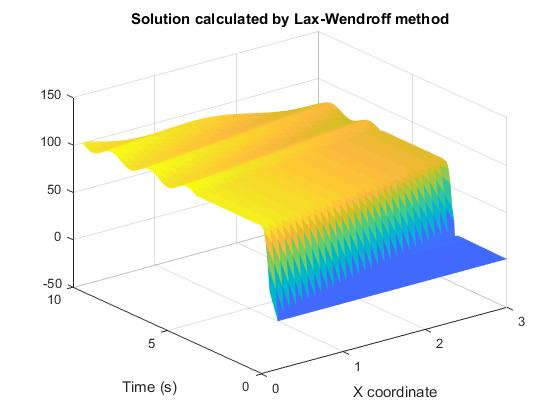
\includegraphics[width=\textwidth,center]{surf2}
\caption{Plots of solution using the Lax Wendroff method}
\end{figure}

This looks very much the same as the plot obtained for the Upwind method. 

\end{document}

%%%Computer Lab 6
clc,clear all,close all
N = 100;
T = 1;
a = 1;
count=1;



for sig = [0.8 1 1.1 ]
       
    
    u1=[];
    u2=[];
    u3=[];
    u1(1,:)=zeros(1,N);
    u2(1,:)=zeros(1,N);
    u3(1,:)=zeros(1,N);
 
    for t=0:sig*2/(N*a):2
      for i=2:N-1
           if  t <= T/2
               u1(count+1,1) = 1;
           elseif t <= T
               u1(count+1,1) = -1;
           elseif t <= 3/2*T
               u1(count+1,1) = 1;
           else
               u1(count+1,1) = -1;
           end

           if  t <= T/2
               u2(count+1,1) = 1;
           elseif t <= T
               u2(count+1,1) = -1;
           elseif t <= 3/2*T
               u2(count+1,1) = 1;
           else
               u2(count+1,1) = -1;
           end

           if  t <= T/2
               u3(count+1,1) = 1;
           elseif t <= T
               u3(count+1,1) = -1;
           elseif t <= 3/2*T
               u3(count+1,1) = 1;
           else
               u3(count+1,1) = -1;
           end

         u1(count+1,i)=(1-sig)*u1(count,i)+sig*u1(count,i-1); %Upwind
         u2(count+1,i)=0.5*(u2(count,i-1)+u2(count,i+1))-0.5*sig*(u2(count,i+1)-u2(count,i-1)); %Lax-Friedrich
         u3(count+1,i)=u3(count,i)-0.5*sig*(u3(count,i+1)-u3(count,i-1))+0.5*sig^2*(u3(count,i+1)-2*u3(count,i)+u3(count,i-1)); %Lax-Wendroff
      end
      u1(count+1, N)=(1-sig)*u1(count,N)+sig*u1(count,N-1);
      u2(count+1, N) = 2*u2(count+1, N-1) - u2(count+1, N-2);
      u3(count+1, N) = 2*u3(count+1, N-1) - u3(count+1, N-2);
      count=count+1;
   end
   figure
   subplot(1,3,1)
   plot(2/N*(1:N), u1(end,:))
   title(['Upwind \sigma =' num2str(sig)])
   xlabel('x')
   ylabel('u(x,2T)')
   
   subplot(1,3,2)
   plot(2/N*(1:N), u2(end,:))
   title(['Lax-Friedrich \sigma =' num2str(sig)])
   xlabel('x')
   ylabel('u(x,2T)')
   
   subplot(1,3,3)
   plot(2/N*(1:N), u3(end,:))
   title(['Lax-Wendroff \sigma =' num2str(sig)])
   xlabel('x')
   ylabel('u(x,2T)')
   
end





%% PART b)%%
clc,clear all,close all
%Constants
L=3; a2=0.1; v=1; Tcool=5; Thot=100;
M=30;
ht=0.1;
T=[];
T(:,1)=ones(1,M)'*Tcool;
for k=1:100
    if k<=5
    T(1,k) = Tcool+(Thot-Tcool)*sin(pi*(k)/10);
    elseif k<=40
        T(1,k)=Thot;
    else
        T(1,k)=Thot+Tcool*sin(pi*((k)/10-4));
    end
for i=2:M
    T(i,k+1)=(1-ht*a2)*T(i,k)-(T(i,k)-T(i-1,k))+ht*a2*Tcool;
end

end
T(1,101)=Thot+Tcool*sin(pi*((100)/10-4));

[xMesh, tMesh] = meshgrid(ht:ht:L, 0:ht:tend*ht);
surf(xMesh, tMesh, T',  'EdgeColor', 'none')
title('Solution calculated by Lax-Wendroff method')
ylabel('Time (s)')
xlabel('X coordinate ')

%% Lax-Wendroff
L=3; a=0.1; v=1; Tcool=5; Thot=100;
M=30;
ht=0.1;
T=[];
tend = 100;
T(:,1)=ones(1,M)'*Tcool;
T=ones(M,tend+1);
for k=1:tend
    if k<=5
    T(1,k) = Tcool+(Thot-Tcool)*sin(pi*(k)/10);
    elseif k<=40
        T(1,k)=Thot;
    else
        T(1,k)=Thot+Tcool*sin(pi*((k)/10-4));
    end
%     for i=2:M-2
%         T(i, k+1) = (0.5+0.25-a*ht/2)*T(i-1,k) + (1-ht*a-0.5+a^2*ht^2/2)*T(i,k) + (-0.5+0.25+a*ht/2)*T(i+1,k) + (a*ht-a^2*ht^2/2)*Tcool;
%     end
%     T(M, k) = 2*T(M-1,k)-T(M-2,k);
%     i = M-1;
%     T(i, k+1) = (0.5+0.25-a*ht/2)*T(i-1,k) + (1-ht*a-0.5+a^2*ht^2/2)*T(i,k) + (-0.5+0.25+a*ht/2)*T(i+1,k) + (a*ht-a^2*ht^2/2)*Tcool;
    for i = 2:M-1
        T(i, k+1) = (0.5+0.5-a*ht/2)*T(i-1,k) + (-ht*a+a^2*ht^2/2)*T(i,k) + (-0.5+0.5+a*ht/2)*T(i+1,k) + (a*ht-a^2*ht^2/2)*Tcool;
    end
    T(M,k+1) = 2*T(M-1,k+1) - T(M-2,k+1);
end
T(1,tend+1)=Thot+Tcool*sin(pi*((tend)/10-4));
%surf(T, 'EdgeColor', 'none')

[xMesh, tMesh] = meshgrid(ht:ht:L, 0:ht:tend*ht);
surf(xMesh, tMesh, T',  'EdgeColor', 'none')
title('Solution calculated by Lax-Wendroff method')
ylabel('Time (s)')
xlabel('X coordinate ')